\section{Newly generated real-model evidence}
\label{sec:real}
\subsection{Frozen search and fresh-question audit}
We newly generated Qwen2.5-1.5B-Instruct Q4\_K\_M answers on pinned MMLU-Pro, using greedy CPU inference and a strict, frozen capital-letter parser. The benchmark has 12,032 test questions in 14 categories, with 3--10 options. Validation questions checked implementation and timing. Neither gold answers nor rationales entered generation. Four instruction/format candidates, including default 0, were searched on 256 questions; 512 disjoint questions provide the audit. The primary matrix contains 3,072 answers. An outcome-blind, prespecified calendar rule reduced the original design after a completed eight-candidate shard; all 6,144 generated answers are preserved and costed. Appendix~\ref{app:real-protocol} records the freeze, fallback, exact inference and compute. The target is the 11,776-question complement defined in Section~\ref{sec:methods}, not full-benchmark or unrestricted future-task accuracy.

Figure~\ref{fig:real-primary} shows the unique search winner, candidate 10: 94/256, or 36.72\%, compared with 130/512, or 25.39\%, on audit. Its adjusted exact audit interval is [21.27,29.87]\%; the observed reuse--audit gap is 11.33 pp, with interval [6.85,15.45] pp for reused score minus remaining-benchmark accuracy. The transformed simultaneous-search interval for remaining-benchmark accuracy is [28.55,45.46]\%. These finite-population intervals have the two-design unconditional guarantees specified above, separately per endpoint family; one realization cannot measure coverage.

Crucially, default 0 also drops from 25.39\% search to 16.80\% audit, a gap of 8.59 pp. The winner's excess gap beyond that default gap is only 2.73 pp, with adjusted interval [$-2.81$,8.45] pp. Thus the entire 11.33 pp cannot be identified as selection-only optimism. A single partition does not distinguish sampling variation, optimization, or other explanations of the common gap.

The winner improves over default on paired audit questions: 61 wins and 17 losses give +8.59 pp, with adjusted exact paired interval [2.88,14.14] pp. The conservative ordinary reused-interval nonoverlap rule does \emph{not} declare superiority; the adjusted audit nonoverlap rule does, and the paired audit lower bound is positive. Reporting changes the decision toward audit-supported improvement here. This is not an observed false-positive reuse decision, nor an estimate of population false-superiority risk.


\begin{figure}[t]
\centering
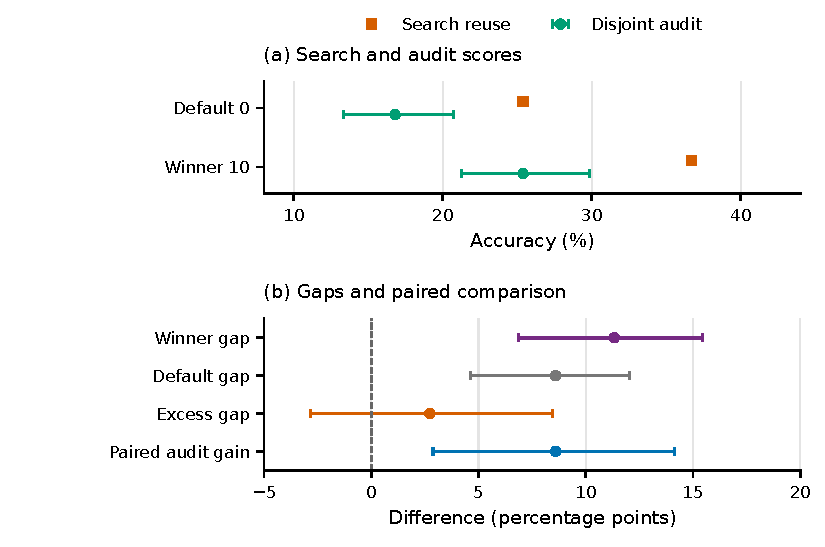
\includegraphics[width=\linewidth]{figures/real-primary.pdf}
\caption{\textbf{The default shares much of the winner's search--audit gap.} Qwen 2.5-1.5B-Instruct on MMLU-Pro; four frozen candidates, 256 search and 512 disjoint audit questions. (a) Squares: search scores; circles: audit estimates of accuracy on the 11,776-question reservoir complement. (b) Search-minus-audit gaps, their difference (excess gap), and paired winner-minus-default audit gain. The winner gap is 11.33 pp versus the default's 8.59 pp; the excess-gap interval crosses zero, so the full gap cannot be identified as selection-only optimism. Whiskers use exact finite-population endpoints with error .025 per possible runtime design: at least 95\% unconditional protection separately per endpoint family, without a joint-all-endpoint or conditional-on-trigger guarantee. This is one realized partition. The paired gain supports improvement; the primary reporting/decision/cost table gives the distinct comparison rules.}
\label{fig:real-primary}
\end{figure}

\subsection{Reselection and reporting calibration}
We repeat selection 20,000 times in each of 15 $n/K$ cells, $n\in\{16,32,64,128,256\}$ and $K\in\{1,2,4\}$, conditional on the same search/audit matrices. At $K=4$, mean reuse--audit gaps are 14.59, 11.55 and 11.33 pp for $n=16,64,256$; $K=1$ retains the default's approximately 8.59 pp gap. MCSE describes conditional computation, not fresh-pool uncertainty. A paired-row bootstrap independently resamples both pools and reruns selection (1,000 outer, 2,000 inner repetitions). Its approximate 95\% sensitivity range for the gap at $n=256,K=4$ is [4.69,18.55] pp. These ranges do not replace exact audit uncertainty or supply runtime-conditional coverage.

For a separate known-truth experiment, we sample whole rows iid with replacement from the retained 768-question/four-candidate cache. The selected candidate's exact cache mean is the target. Figure~\ref{fig:real-cache} summarizes calibration; 20,000 repetitions per cell evaluate all five reporting protocols from Section~\ref{sec:methods}. At $K=4$, reuse optimism decreases from 4.97 pp (MCSE 0.075) at $n=16$ to 0.214 pp (MCSE 0.020) at $n=256$.

Ordinary nominal 95\% coverage across all 15 cells is \mbox{95.290--97.585\%}: this small real bank exhibits positive point bias \emph{without observed nominal undercoverage}. It does not reproduce the large-bank synthetic coverage failure.

At $n=256,K=4$, ordinary, simultaneous and independent-audit coverage is 95.425\%, 98.905\% and 95.510\%, with mean widths 11.46, 14.46 and 11.43 pp. Simultaneous protection is conservative and widens without changing point bias. Full-search selected cache quality is 29.02\%, compared with 28.75\% under half-question splitting and 28.94\% under equal-call splitting; these are their respective winners' qualities. Reuse uses 1,024 logical calls, extra auditing 1,280, question splitting 640, and call splitting 1,024. These calibration budgets differ from the primary disjoint audit and actual generation costs. The largest per-cell false-superiority frequency is one in 20,000 (naive reuse); zero events still allow a per-cell one-sided 95\% upper risk of 0.015\%.


\begin{figure}[t]
\centering
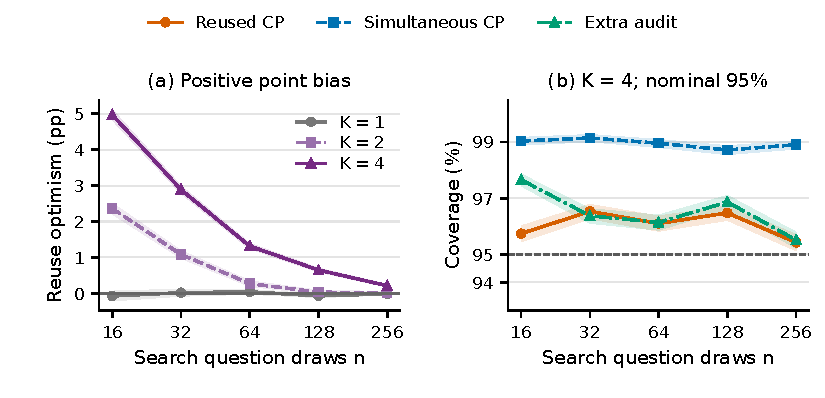
\includegraphics[width=\linewidth]{figures/real-cache-main.pdf}
\caption{\textbf{Positive point bias coexists with no observed nominal undercoverage in this small bank.} Whole paired rows from the 768-question/four-candidate cache are drawn iid with replacement; full selection/reporting is repeated 20,000 times per cell. Truth is the selected candidate's exact empirical-cache mean. (a) Reuse optimism by frozen-prefix bank size K. (b) Coverage of nominal 95\% Clopper--Pearson (CP) reporting at K=4; dashed line: 95\%. Bands are marginal 95\% computational intervals (mean $\pm$ 1.96 MCSE for optimism, exact binomial for coverage), conditional on this cache. Reuse coverage is 95.290--97.585\% across all 15 cells. This calibration target differs from remaining-benchmark accuracy in the primary display. Simultaneous CP keeps the reused point score; extra audit uses n additional question draws/calls. Full five-method coverage, widths, selection quality, score error, decisions and budgets accompany the appendix.}
\label{fig:real-cache}
\end{figure}

\paragraph{Diagnostics and scope.}
The retained responses include 398 malformed answers (12.96\%) and no out-of-range letters. Winner 10 has none; default 0 has 164/768. Format adherence is part of the measured system, so improvements cannot be interpreted purely as knowledge gains. All contexts fit. Candidate correctness correlations span 0.531--0.699; this descriptive range does not identify a causal dependence effect. Category results retain explicit denominators and question weighting. All raw responses, complete driver/calibration grids, uncertainty, diagnostics and costs accompany the code.

Appendix~\ref{app:real-evidence} gives the full grids, numerical decision/cost comparisons, sensitivity ranges and diagnostics.
